%Main
\documentclass{beamer}
\usepackage[utf8]{inputenc}

\author{Jan Lukas Deichmann, Veith Güntel}
\title{Betriebssysteme WS15/16}
\date{\today}

\begin{document}
%1
\maketitle
%2
\frame{\tableofcontents}

%3
\section{Demo}
\begin{frame}
\frametitle{Demo}
\begin{figure}[!h]
    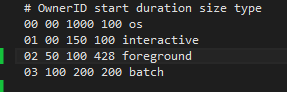
\includegraphics[scale=0.3]{processes}
    \caption{processes.txt}
\end{figure}
\end{frame}

%4
\section{Getroffene Annahmen}
\begin{frame}
\frametitle{Getroffene Annahmen}
\begin{itemize}
	\item Kein Prozess bekommt jemals PID 0 vom System zugewiesen.
	\item Es wird kein Prozess gestartet der größer als der Systemspeicher ist.
\end{itemize}
\end{frame}

%5
\section{Funktionsumfang}
\begin{frame}
\frametitle{Funktionsumfang}
Erweiterung von SimOS um:
\begin{itemize}
	\item \textbf{Process Queue} zur verwaltung von Prozessen die aktuell nicht in den Speicher passen.
	\item \textbf{Memory List} zum Speichermanagement.
\end{itemize}
\end{frame}

%6
\section{Entwurfsentscheidungen}
\begin{frame}
\frametitle{Entwurfentscheidungen}
\begin{itemize}
	\item \textbf{Auswahlstrategie} für Speicherallozierung ist First-Fit.
	\item \textbf{Speichermanagement} als verkettete Liste.
	\item \textbf{Process Management} als Queue.
	\item \textbf{Kompaktierungszeitpunkt} immer dann, wenn ein Prozess nicht passt.
\end{itemize}
\end{frame}
\end{document}